\documentclass[12pt, oneside, a4paper]{article}
% PREÂMBULO - CONFIGURAÇÕES ABNT (CLASSE ARTICLE)
% ====================================================
% \usepackage{abntex2}
\usepackage[utf8]{inputenc}
\usepackage[T1]{fontenc}
% \usepackage[brazilian]{babel}
\usepackage{lipsum}
\usepackage{times}
\usepackage{geometry}
\usepackage{setspace}
\usepackage[alf,abnt-emphasize=bf]{abntex2cite}
\usepackage{titlesec}
\usepackage{titletoc}
\usepackage{caption}
\usepackage{etoolbox}
\usepackage{amsmath}
\usepackage{changepage}
\usepackage{ragged2e}
\usepackage{siunitx}

\setlength{\headheight}{14.5pt}

% --- PACOTES GRÁFICOS ESSENCIAIS ---
\usepackage{graphicx} % Figuras básicas
\usepackage{float}    % Posicionamento preciso
\usepackage{booktabs} % Tabelas profissionais
\usepackage{subcaption} % Subfiguras
\usepackage{caption} % Subfiguras
\usepackage{pgfplots}  % Gráficos avançados
\pgfplotsset{compat=1.18}
\usepackage{tikz}      % Diagramas vetoriais
\usepackage{multicol}

% --- MARGENS ABNT ---
\geometry{a4paper,left=3cm,right=2cm,top=3cm,bottom=2cm}

\onehalfspacing                 % Espaçamento 1,5 linha (ABNT)

% --- RECUO E ESPAÇAMENTO PADRÃO ABNT ---
\setlength{\parindent}{1.25cm} % Recuo de parágrafo
\setlength{\parskip}{0pt} % Remove espaço extra entre parágrafos
\raggedbottom % Evita espaçamento irregular


\usepackage{fancyhdr}
\fancyhf{} % limpa todos os campos do cabeçalho e rodapé
\fancyhead[R]{\thepage} % número da página à direita no topo
\renewcommand{\headrulewidth}{0pt} % remove linha horizontal do topo
\renewcommand{\footrulewidth}{0pt} % remove linha no rodapé

% Configuração da fonte
\renewcommand{\paragraph}{\fontsize{12}{14}\selectfont} % Tamanho 12 com espaçamento 1.5

% --- CORREÇÃO DO RECUO NO PRIMEIRO PARÁGRAFO ---
\usepackage{indentfirst} % Garante recuo mesmo no primeiro parágrafo
\setlength{\parindent}{1.25cm} % Recuo ABNT padrão

% --- FORMATAÇÃO DAS SEÇÕES (ABNT) ---
\usepackage{titlesec}

% Seções (Nível 1)
\titleformat{\section}
  [hang] % alinhado à esquerda
  {\normalfont\bfseries\fontsize{12}{14}\selectfont\MakeUppercase}
  {\thesection}{1em}{}


% Subseções (Nível 2)
\titleformat{\subsection}
  [hang]
  {\normalfont\fontsize{12}{14}\selectfont}
  {\thesubsection}{1em}{}


% Subsubseções (Nível 3)
\titleformat{\subsubsection}
  [hang]
  {\normalfont\fontsize{12}{14}\selectfont}
  {\thesubsubsection}{1em}{}

% --- COMANDO PERSONALIZADO PARA "CAPÍTULOS" NÃO NUMERADOS ---
\newcommand{\capitulo}[1]{
  \begin{center}
    \vspace{2em}
    \textbf{\MakeUppercase{#1}}
    \vspace{1em}
  \end{center}
}


% Espaçamento vertical
\titlespacing*{\section}{0pt}{18pt}{6pt}    % [left]{before}{after}
\titlespacing*{\subsection}{0pt}{12pt}{6pt}
\titlespacing*{\subsubsection}{0pt}{12pt}{6pt}

% Profundidade de numeração
\setcounter{secnumdepth}{3} % Até subsubseções

\usepackage[titles]{tocloft}

% --- FORMATAÇÃO DO SUMÁRIO ---
% \usepackage{tocloft}
% \usepackage[nottoc]{tocbibind} % Evita que o título "Sumário" apareça no próprio sumário
\renewcommand{\contentsname}{\begin{center}
        \bfseries\MakeUppercase{Sumário}
      \end{center}}
% Recuo das seções (ABNT padrão: sem recuo)
\titlecontents{section}[1.5em]           % Recuo da seção
{\addvspace{0pt}\bfseries\normalsize}  % Estilo
{\contentslabel{1.5em}}                % Alinhamento do número
{}                                     % Sem recuo adicional
{\titlerule*[0.6pc]{.}\contentspage}   % Pontilhado e número de página


% Recuo das subseções (ligeiramente menor)
\titlecontents{subsection}[1.5em]
{\normalfont\normalsize}
{\contentslabel{1.5em}}
{}
{\titlerule*[0.6pc]{.}\contentspage}



% Centraliza e coloca em maiúsculas a lista de figuras
\renewcommand{\listfigurename}{
  \bfseries\MakeUppercase{Figuras}}

% Centraliza e coloca em maiúsculas a lista de tabelas
\renewcommand{\listtablename}{\begin{center}
  \bfseries\MakeUppercase{Lista de Tabelas}
\end{center}}

% --- CONFIGURAÇÕES DE FIGURAS E TABELAS ---
\captionsetup[figure]{
  position=above,    % Legenda acima da figura
  justification=centering,
  labelsep=endash,
  name=Figura,
  font=small,
  labelfont=bf
}

% Comando personalizado para fonte abaixo
\newcommand{\fonte}[1]{
  \vspace{-0.5em} % Ajuste de espaçamento
  \begin{center}
    \footnotesize\textbf{Fonte:} #1
  \end{center}
}

% --- CONFIGURAÇÃO DE TABELAS ABNT ---
\captionsetup[table]{
  position=above,     % Legenda acima da tabela
  justification=centering,
  labelsep=endash,
  name=Tabela,
  font=small,
  labelfont=bf
}

\newcommand{\fontet}[1]{
  \begin{center}
    \footnotesize\textbf{Fonte:} #1
  \end{center}
}

% Comandos personalizados para o formato ABNT
\DeclareCaptionLabelFormat{abntformat}{\textbf{#1~#2}}
\captionsetup[figure]{labelformat=abntformat}
\captionsetup[table]{labelformat=abntformat}

\usepackage{tocloft}

% --- CONFIGURAÇÕES PARA LISTA DE FIGURAS ---
\setlength{\cftfigindent}{0pt}
\setlength{\cftfignumwidth}{6em}
\renewcommand{\cftfigpresnum}{\textbf{FIGURA~}}
\renewcommand{\cftfigaftersnum}{\textbf{~--~}}
\renewcommand{\cftfigdotsep}{3}

% --- CONFIGURAÇÕES PARA LISTA DE TABELAS ---
\setlength{\cfttabindent}{0pt}             % Sem recuo
\setlength{\cfttabnumwidth}{6em}           % Espaço reservado para "TABELA 10"
\renewcommand{\cfttabpresnum}{\textbf{TABELA~}}  % Prefixo
\renewcommand{\cfttabaftersnum}{\textbf{~--~}}   % Sufixo
\renewcommand{\cfttabdotsep}{3}            % Mais pontos entre nome e número de página



% Define novo tipo de float
% \newfloat{myequation}{htbp}{loe}
% \floatname{myequation}{EQUAÇÃO}

% % Configura legenda do float
% \captionsetup[myequation]{
%   labelfont=bf,
%   labelsep=space,
%   justification=centering,
%   singlelinecheck=false
% }

% Ambiente "simbolos" no estilo ABNT
\usepackage{enumitem}

\newlist{simbolos}{description}{1}
\setlist[simbolos]{%
  labelwidth=1cm,        % Largura da coluna do símbolo
  labelsep=1cm,          % Espaço entre símbolo e descrição
  leftmargin=2cm,        % Recuo à esquerda (soma de labelwidth + labelsep)
  style=nextline,        % Quebra de linha após o símbolo
  font=\normalfont       % Fonte normal no símbolo
}

% Cria a lista de gráficos
\newlistof{grafico}{lol}{Gráficos}

% Formatação da numeração da legenda no corpo do documento
\renewcommand{\thegrafico}{\arabic{grafico}}

% Formatação da numeração na lista de gráficos (prefixo em maiúsculas e negrito)
\renewcommand{\cftgraficopresnum}{\textbf{GRÁFICO~}}
\renewcommand{\cftgraficoaftersnum}{\textbf{~--~}}  % traço com espaços antes e depois
\setlength{\cftgraficonumwidth}{7em}      % largura reservada para o número
\setlength{\cftgraficoindent}{0pt}        % sem indentação extra

% Configura legenda para o tipo 'grafico'
\captionsetup[grafico]{
  position=above,
  justification=centering,
  labelsep=endash,
  font=small,
  labelfont=bf,
  name=Gráfico,
  labelformat=simple
}

\setcounter{grafico}{0}

% Comando para inserir gráfico com legenda acima, fonte abaixo e label
\newcommand{\inserirgrafico}[5][]{%
  \begin{center}
    \captionsetup{type=grafico,position=above}%
    \captionof{grafico}{#3}%
    \label{#5}% label logo após a legenda
    \includegraphics[#1]{#2}%
    \par\vspace{0.1em}%
    {\footnotesize\textbf{Fonte:} #4}%
  \end{center}
}

% Define o nome da lista de equações
\newcommand{\listequationsname}{Equações}

% Cria a lista de equações com extensão .loe
\newlistof{equationlist}{loe}{\listequationsname}

% Prefixo e sufixo na lista de equações (prefixo em negrito e traço)
\renewcommand{\cftequationlistpresnum}{\textbf{EQUAÇÃO~}}
\renewcommand{\cftequationlistaftersnum}{\textbf{~--~}}
\setlength{\cftequationlistnumwidth}{7em}
\setlength{\cftequationlistindent}{0pt}

% Comando para adicionar entrada na lista de equações
% #1 = texto da entrada na lista (normalmente a equação ou descrição)
\newcommand{\addtoequationlist}[1]{%
  \addcontentsline{loe}{equationlist}{\protect\numberline{\theequation}#1}%
}





% --- Ambiente Personalizado ErrataABNT ---
% ==== NO PREÂMBULO ====  
\usepackage{geometry}   % para controle de margem  
\usepackage{setspace}   % espaçamento  
\usepackage{array}      % para tabelas  
\usepackage{caption}    % legendas  

% Comando para inserir a página de Errata ABNT
\newcommand{\paginaErrata}[1]{%
  \clearpage
  \thispagestyle{empty}         % sem cabeçalho/rodapé  
  \newgeometry{left=1cm, right=2cm, top=3cm, bottom=2cm}  
  \section*{\begin{center}Errata\end{center}}        % título senúmero  
  % \vspace{1\baselineskip}  
  \setstretch{1.0}               % espaçamento simples  
  % ==== TABELA DE ERROS ====  
  {\renewcommand{\arraystretch}{1.5}% altura das linhas
  \input{tabelas/erros}
  % \begin{tabular}{@{} p{2.5cm} p{3cm} p{5cm} p{5cm} @{}}
  %   \hline
  %   \textbf{Folha} & \textbf{Linha} & \textbf{Onde se lê} & \textbf{Leia-se} \\
  %   \hline
  %   10             & 15             & \textit{“esperem resultados imediatos”} & \textit{“esperem resultados mediatos”} \\
  %   45             & 3              & “processo contínuo de ensino e apredizado” & “processo contínuo de ensino e aprendizado” \\
  %   % adicione quantas linhas forem necessárias
  %   \hline
  % \end{tabular}
  }
  \restoregeometry
  \clearpage
}


% --- CONFIGURAÇÕES PARA O SUMÁRIO ---
\setlength{\cftsecindent}{0pt}             % Seções alinhadas à esquerda
\setlength{\cftsecnumwidth}{0em}
\renewcommand{\cftsecleader}{\cftdotfill{\cftdotsep}} % Aplica pontilhado
\renewcommand{\cftdotsep}{3}               % Aumenta pontos do sumário

% (Opcional) para subseções também
\setlength{\cftsubsecindent}{0pt}
\setlength{\cftsubsecnumwidth}{4em}
\renewcommand{\cftsubsecleader}{\cftdotfill{\cftdotsep}}
\renewcommand{\cftdotsep}{3}               % Aumenta pontos do sumário

% Pré-requisitos
\usepackage{graphicx}  % rotatebox
\usepackage{geometry}  % definir dimensões da página

\newcommand{\lombada}[3]{%
  \clearpage
  \newgeometry{left=0cm, top=0cm, bottom=0cm, right=0cm}
  \thispagestyle{empty}

  % Ambiente centralizado vertical com largura total da lombada
  \begin{center}
    \vspace*{1cm} % Espaço até autor (posição vertical)
    \rotatebox{270}{{\textbf{\MakeUppercase{#1}}}} % Autor
    
    \vspace*{2cm} % Espaço até o título (aproximadamente até 15cm do topo)
    \rotatebox{270}{{\textbf{\MakeUppercase{#2}}}} % Título

      % Último item: horizontal, alinhado à esquerda, com largura de 4cm
  \vspace*{2.5cm} % Espaço até parte inferior (29.7 - 26.5 ≈ 3.2)
  \hspace*{0.4cm} % margem esquerda interna da lombada (ajustável)
  \parbox[t]{5cm}{\centering\normalsize\MakeUppercase{#3}}

  \end{center}
  
  \restoregeometry
  \clearpage
}

% Ficha catalográfica formatada segundo a ABNT
\usepackage{geometry} % já deve estar incluso

\newcommand{\fichacatalografica}[9]{%
  \clearpage
  \newgeometry{left=3cm, right=2cm, top=3cm, bottom=2cm}
  \thispagestyle{empty}
  \vspace*{\fill}
  \hspace*{\fill}
  \fbox{%
    \begin{minipage}[t][7.5cm][t]{12.5cm}
      \setstretch{1.0}
      \normalfont\fontsize{12}{14}\selectfont
      \raggedright
      #1\\ % Autor
      \MakeUppercase{#2} / #1. – #3 ed. – #4: #5, #6.\\ p. 35\\
      \textbf{Classificação:} #7\\
      \textbf{ISBN:} #8
      \textbf{CDD:} #9
    \end{minipage}
  }%
  \vspace*{1cm}
  \restoregeometry
  \clearpage
}





% --- FORMATAÇÃO DA BIBLIOGRAFIA ABNT COM TÍTULO CENTRALIZADO, NEGRITO E UPPERCASE ---
\makeatletter
\renewenvironment{thebibliography}[1]
     {
      \begin{center}
        \bfseries\MakeUppercase{Referências}
      \end{center}
      \@mkboth{\MakeUppercase{\refname}}{\MakeUppercase{\refname}}%
      \list{\@biblabel{\@arabic\c@enumiv}}%
           {\leftmargin=0cm
            \labelwidth=0cm
            \labelsep=0cm
            \itemindent=0pt
            \parsep=0pt
            \itemsep=1.5\baselineskip
            \usecounter{enumiv}}%
      \singlespacing
      \sloppy
      \clubpenalty4000
      \@clubpenalty \clubpenalty
      \widowpenalty4000%
      \sfcode`\.\@m
     }
     {\def\@noitemerr
       {\@latex@warning{Empty `thebibliography' environment}}%
      \endlist}
\makeatother

% ====================================================
\begin{document}
\pagestyle{fancy}  % Algarismos romanos minúsculos

% ====================================================
% ELEMENTOS PRÉTEXTUAIS
% ====================================================


\begin{center}
\thispagestyle{empty} 
    % Logo (se necessário)
    % \includegraphics[width=0.9\textwidth]{figuras/image.png}



    \vspace*{0.2cm}
    
    {\normalsize\bfseries INSTITUTO FEDERAL DE EDUCAÇÃO, CIÊNCIA E TECNOLOGIA FLUMINENSE \textit{CAMPUS} BOM JESUS DO ITABAPOANA \\ BACHARELADO EM ENGENHARIA DE COMPUTAÇÃO \\ FÍSICA EXPERIMENTAL II}

    \vspace{3cm}

    % Nome do autor
    {\normalsize PEDRO HENRIQUE ROCHA DE ANDRADE}

    \vspace{7cm}

    % Título
    {\Large\bfseries Prática VI: \\}
    {\normalsize Dilatação Linear}

    \vspace{4cm}

    % Professor
    % {\normalsize Professor: Dr. Rodrigo Lacerda da Silva}

    \vspace{4cm}

    % Local e data
    {\normalsize\ Bom Jesus do Itabapoana -- RJ \\
    2025}

\end{center}

\begin{center}
\thispagestyle{empty} 
    {\normalsize PEDRO HENRIQUE ROCHA DE ANDRADE}

    \vspace{5cm}

    {\Large\bfseries Prática VI: \\}
    {\normalsize Dilatação Linear}
    \vspace{6cm}

    \hspace{6cm}
\begin{flushright}
\begin{minipage}{0.55\textwidth}
    \singlespacing
    Relatório de prática experimental da disciplina de Física Experimental II como parte da avaliação parcial do curso de Bacharelado em Engenharia de Computação, ministrado pelo professor Dr. Rodrigo Lacerda.
    % \\ Orientadora: Profª Dra. Ana Cecília Soja.
\end{minipage}
\end{flushright}

    \vspace{6cm}

    {\normalsize Bom Jesus do Itabapoana -- RJ \\
    2025}

\end{center}
\begin{center}
    \textbf{LISTA DE ILUSTRAÇÕES}
\end{center}
\thispagestyle{empty} 
\listoffigures
\listofgrafico
\listofequationlist
\include{PRETEXTUAIS/tabelas}
\capitulo{Lista de Símbolos}
\thispagestyle{empty} 

\begin{simbolos}
  \item[$\propto $] Proporcional a
  \item[$\alpha $] Coeficiente Angular da Reta
  \item[$\delta $] Erro Experimental
  \item[$\mu $] Densidade Linear de Massa
  \item[$\lambda $] Comprimento de Onda
\end{simbolos}

\include{PRETEXTUAIS/sumario}

% ====================================================
% ELEMENTOS TEXTUAIS
% ====================================================

\pagenumbering{arabic}
\setcounter{page}{6}
\section{INTRODUÇÃO}

A dilatação térmica é um fenômeno físico que descreve a variação nas dimensões de um corpo (sólido, líquido ou gás) quando sua temperatura é alterada. A maioria dos materiais se expande quando aquecida e se contrai quando resfriada. Este fenômeno é de suma importância em diversas aplicações de engenharia, desde a construção de pontes e ferrovias até o design de componentes eletrônicos.

No caso dos sólidos, a dilatação pode ser linear, superficial ou volumétrica. A dilatação linear, foco deste experimento, refere-se à mudança no comprimento de um material. Teoricamente, a variação de comprimento $\Delta L$ de um material sólido com um comprimento inicial $L_0$ submetido a uma variação de temperatura $\Delta T$ é dada pela relação:
\begin{equation}
\Delta L = \alpha \cdot L_0 \cdot \Delta T
\label{eq:dilatacao_linear}
\end{equation}
\addtoequationlist{Dilatação Linear}
Onde $\alpha$ é o coeficiente de dilatação linear, uma propriedade intrínseca de cada material que quantifica sua tendência a dilatar ou contrair. Materiais diferentes possuem coeficientes de dilatação linear distintos. A unidade de $\alpha$ é tipicamente por grau Celsius ($^\circ C^{-1}$) ou por Kelvin ($K^{-1}$).

Este experimento, conforme ilustrado na Figura \ref{fig:esquema_montagem}, tem como objetivo determinar o coeficiente de dilatação linear ($\alpha$) de diferentes materiais (latão, alumínio e aço) através da medição da variação de comprimento de tubos metálicos quando aquecidos por vapor d'água. A comparação dos valores experimentais com os valores tabelados nos permitirá calcular o erro relativo, avaliando a precisão do nosso método.

\begin{figure}[H]
    \centering
    \caption{Esquema de montagem do Dilatômetro}
    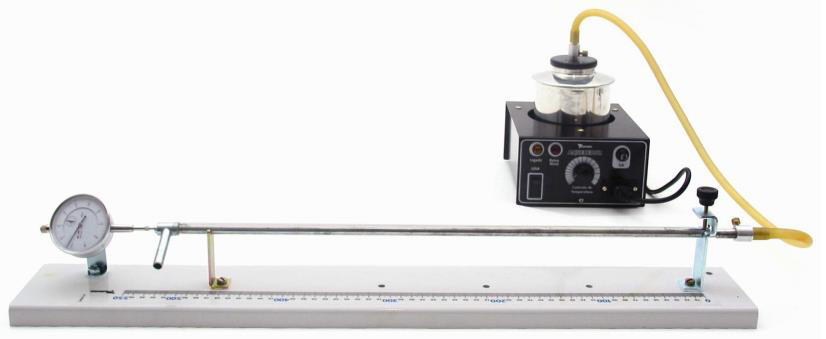
\includegraphics[width=0.7\linewidth]{figuras/esquema.png}
    \fonte{\citeonline{roteiro}}
    \label{fig:esquema_montagem}
\end{figure}

Os objetivos específicos deste experimento são:
\begin{enumerate}
    \item Realizar a montagem do dilatômetro e operar o gerador de vapor de forma segura e eficaz.
    \item Medir o comprimento inicial, as temperaturas inicial e final, e a dilatação dos corpos de prova de diferentes materiais.
    \item Calcular o coeficiente de dilatação linear ($\alpha$) para cada material com base nas medições.
    \item Comparar os valores experimentais de $\alpha$ com os valores tabelados e determinar o erro relativo.
    \item Discutir as fontes de incerteza e possíveis melhorias no procedimento experimental.
\end{enumerate}
\section{MATERIAIS E MÉTODOS}

\subsection{Materiais Utilizados}

Para o experimento foram utilizados os seguintes materiais e equipamentos:
\begin{itemize}
    \item Gerador de ondas/sinais;
    \item Mola helicoidal (longitudinal);
    \item Suporte de ferro;
    \item Mufas embutidas;
    \item Pinça com mufa;
    \item Dinamômetro;
    \item Estroboscópio;
    \item Haste para suporte;
    \item Suporte para mola (acoplado à haste);
    \item Trena.
\end{itemize}

\subsection{Procedimentos Experimentais}

A montagem experimental foi configurada para a geração e observação de ondas longitudinais estacionárias em uma mola. Um suporte de ferro foi conectado ao gerador de ondas utilizando mufas. Na parte superior do suporte, uma pinça com mufa foi acoplada, à qual um dinamômetro de 2N foi preso. Uma extremidade da mola foi fixada ao pino do gerador de ondas, enquanto a outra extremidade foi conectada ao dinamômetro. A figura \ref{fig:esquema} ilustra o esquema.

\begin{figure}[H]
    \centering
    \caption{Esquema do sistema de ondas longitudinais}
    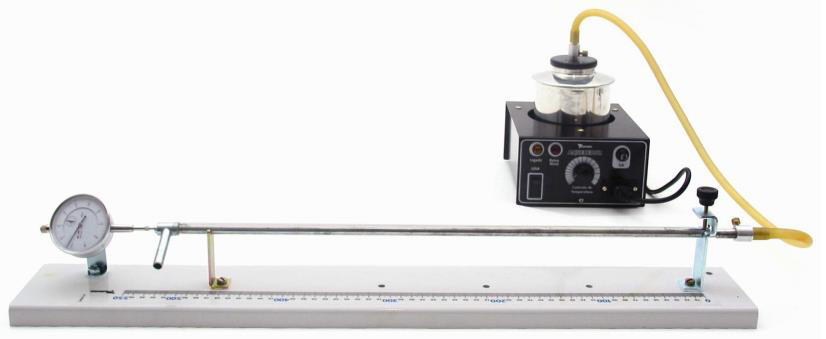
\includegraphics[width=0.15\linewidth]{figuras/esquema.png}
    \label{fig:esquema}
    \fonte{\citeonline{roteiro}}
\end{figure}

O gerador foi configurado para operar como gerador de sinais, com a chave seletora ajustada para a tensão local. Um estroboscópio foi conectado ao gerador de sinais e fixado em uma haste para auxiliar na visualização do fenômeno.



\subsubsection*{Parte I: Definição da Tensão e Observação dos Modos de Vibração}

O procedimento iniciou com a definição de uma tensão inicial na mola por meio do dinamômetro, o que estabeleceu uma altura específica para a mola. Após esta definição, uma mufa com suporte para mola foi acoplada à haste, e a mola foi presa nesse suporte no ponto correspondente à altura desejada, fixando o comprimento efetivo da mola para as medições.

Com o sistema ligado e funcionando, o volume foi ajustado enquanto a frequência do gerador de sinais era variada. Este ajuste permitiu a observação da formação de ondas estacionárias e a identificação dos nós e ventres. 

\subsubsection*{Parte II: Coleta de Dados para Diferentes Tensões}

O experimento foi conduzido para, no mínimo, duas tensões distintas na mola ($T_1$ e $T_2$). Para cada tensão definida, a mola foi fixada através do suporte. Em cada uma dessas condições de tensão, a frequência de ressonância ($F_n$) foi determinada para os diferentes modos de vibração observados. Durante o processo, foi observada a relação entre a variação da tensão e o número de nós formados.

Os dados de frequência de ressonância ($F_n$) e o índice do modo de vibração ($n$) foram registrados em tabelas separadas para cada tensão. Cada entrada da tabela incluiu um esboço da forma da onda observada para o modo correspondente.

% \subsubsection*{Parte III: Análise de Dados Preliminar}

A análise dos dados envolveu a construção de gráficos de $F_n$ versus $n$ para cada uma das tensões ($T_1$ e $T_2$), sendo ambas as curvas plotadas no mesmo gráfico para comparação. A determinação da velocidade de propagação da onda ($v$) para cada tensão foi realizada a partir da análise desses gráficos, empregando a técnica de regressão linear para extrair a inclinação da reta, que está diretamente relacionada à velocidade de propagação.
\section{RESULTADOS E DISCUSSÕES}

\subsection{Coleta de Dados e Frequências de Ressonância}

% \begin{multicols}{2}
\begin{table}[H]
\centering
\caption{Medidas experimentais $T_1$ }
\begin{tabular}{cc}
\toprule
\textbf{n} & \textbf{$F_n$ (Hz)}\\
\midrule
        1   & 7,0        \\
        2   & 15,0       \\
        3   & 20,6       \\
        4   & 28,0       \\
        5   & 34,2       \\
\bottomrule
\end{tabular}
\label{tab:t1}
\fontet{Autoria própria (2025)}
\end{table}
\begin{table}[H]
\centering
\caption{Valores tabelados}
\begin{tabular}{cc}
\toprule
\textbf{Material} & \textbf{Valor ($10^{-5}$ $^{\circ}\text{C}^{-1} $)} \\
\midrule
Ferro & 1,2 \\
Latão & 2,0 \\
Alumínio & 2,2 \\
\bottomrule
\end{tabular}
\label{tab:t2}
\fontet{\citeonline{roteiro}}
\end{table}
% \end{multicols}

\subsection{Análise Gráfica e Determinação da Velocidade de Propagação}



% \inserirgrafico[width=0.8\linewidth]{figuras/grafico1.png}{Frequência ($F_n$) versus índice ($n$) para tensões $T_1$ e $T_2$}{Software SciDAVis (2025)}{graf:grafico1}

\begin{equation}
v = 2 \times L \times \alpha
\label{eq:velocidadecalc}
\end{equation}
\addtoequationlist{Velocidade}

\begin{equation}
\delta v = 2 \times L \times \delta_\alpha
\label{eq:errovelocidade}
\end{equation}
\addtoequationlist{Erro Velocidade}

Os valores obtidos para as velocidades de propagação foram:
\[
\boxed{
v_1 = (7,8 \pm 0,2)\, \text{m/s}
}
\]
\[
\boxed{
v_2 = (9,2 \pm 0,4)\, \text{m/s}
}
\]

\subsection{Discussão dos Resultados}
\section{CONCLUSÃO}

A seção de Conclusão do Experimento deve sumarizar os achados, discutir se os objetivos foram alcançados e analisar as possíveis fontes de erro e limitações do experimento.

Com base nos resultados simulados na Tabela \ref{tab:t1}, os coeficientes de dilatação linear experimentais para latão, alumínio e aço (ferro) foram \SI{2.00e-5}{\degree C^{-1}}, \SI{2.20e-5}{\degree C^{-1}} e \SI{1.20e-5}{\degree C^{-1}} , respectivamente. Na simulação, observou-se uma correspondência perfeita com os valores tabelados, resultando em erros relativos nulos.

Em um cenário experimental real, desvios dos valores tabelados são comuns e esperados. As fontes de erro podem incluir:
\begin{itemize}
    \item Imprecisões nas leituras do relógio comparador, possivelmente devido a erros de paralaxe.
    \item Erros na medição do comprimento inicial $L_0$.
    \item Variações na temperatura ambiente e na temperatura de ebulição da água, que é influenciada pela pressão atmosférica local.
    \item Perda de calor para o ambiente durante o aquecimento do tubo, que pode fazer com que a temperatura média do tubo seja ligeiramente inferior à temperatura do vapor.
    \item Imprecisões na calibração dos instrumentos de medição.
\end{itemize}
Para aprimorar a precisão do experimento, algumas medidas poderiam ser implementadas:
\begin{itemize}
    \item Realizar múltiplas medições para cada material e calcular a média, o que ajuda a mitigar o impacto de erros aleatórios.
    \item Empregar instrumentos de medição com maior precisão e menor incerteza intrínseca.
    \item Isolar termicamente o tubo durante o processo de aquecimento para minimizar a perda de calor.
    \item Levar em consideração a pressão atmosférica local para determinar o ponto de ebulição exato da água.
\end{itemize}
Apesar das potenciais fontes de erro, este experimento proporciona uma compreensão fundamental da dilatação linear e da importância dos coeficientes de dilatação para diferentes materiais, validando o modelo teórico apresentado.


% ====================================================
% ELEMENTOS POSTEXTUAIS
% ====================================================

\bibliographystyle{abntex2-alf}
\nocite{moyses2014, halliday2016, roteiro, scidavis}
\bibliography{referencias}
\addcontentsline{toc}{section}{REFERÊNCIAS}

\end{document}